%% =====================================================================
%%  约束层 —— 自主智能体、确定性账本与机器后果的缺失基底（中文对照稿）
%%
%%  编译：xelatex main_zh.tex（运行两遍）；需 ctex 宏包（TeX Live / MiKTeX）
%%  说明：arXiv 正式投稿以英文版 paper/en/main.tex 为准，本稿为对照版本
%% =====================================================================
\documentclass[11pt,UTF8]{ctexart}

\usepackage[margin=1in]{geometry}
\usepackage{amsmath,amssymb}
\usepackage{booktabs}
\usepackage{graphicx}
\usepackage{caption}
\usepackage{enumitem}
\usepackage{xcolor}
\usepackage[numbers,sort&compress]{natbib}
\usepackage[colorlinks=true,linkcolor=black,citecolor=black,
            urlcolor={blue!35!black}]{hyperref}
\usepackage{xurl}

\captionsetup{font=small,labelfont=bf,width=0.94\textwidth}
\setlist{itemsep=2pt,topsep=4pt}
\emergencystretch=1.5em
\pagestyle{plain}

\hypersetup{
  pdftitle={约束层：自主智能体、确定性账本与机器后果的缺失基底},
  pdfauthor={Xinhao Zheng},
}

\newcommand{\R}[1]{R#1}

\title{\heiti 约束层：\\[3pt]
  自主智能体、确定性账本，与机器后果的缺失基底}
\author{%
  Xinhao Zheng\thanks{通讯邮箱：\texttt{xinhaozheng.vx@outlook.com}。代码与数据：
    \url{https://github.com/xinhao-zheng/constraint-layer}。本稿为中文对照版本；arXiv 正式投稿以英文版为准。}\\[2pt]
  \small 独立研究者}
\date{2026 年 6 月 12 日}

\begin{document}
\maketitle

\begin{abstract}
\noindent
一个自主软件智能体如今能够决策，却无法绑定。当前的模型会规划一笔交易、起草一
份合同、下达一条支付指令，但它所产出的任何东西本身都不可问责：其行为是非确定
性的，它没有抵押，它无法证明自己停留在被授予的权限之内，也无法使任何结果不可
逆。这一缺口是结构性的，而非规模问题——更强的模型决策更好，却并不因此变得可
绑定。我们论证：所缺的这项能力——受规则约束的、可证明的、可清算的后果——恰
恰是某一类公共账本所供给的；二者是互补而非竞争：生成式系统恰恰在账本僵硬而受
规则治理之处开放而不受约束，而对承载后果的自主性而言，二者缺一不可。我们给出
这一缺口的解剖；陈述一个账本要充当智能体的\emph{约束层}必须同时满足的五项性
质——可证安全的共识；使「本地核查的动作等于全局清算的动作」的确定性结算；表
达力足以承载私密合规谓词的证明；为中立性付费却不产生所有者的经济；以及能够自
我修订的规则——并说明为何主流账本设计至多只满足其中若干项。随后，我们以一个
已部署的架构对照这五项做个案分析，依据是架构设计而非市场表现，并描述当权限被
编译为可核查的策略、结算本身即为审计时，智能体商业所呈现的形态。两种常被一并
归为风口的技术，实为同一缺失原语的两半：会决策的机器，以及一个能让其决策承载
后果的基底。决策正在变得充裕；后果尚未；而构建后者，才是更难、也更被忽视的那
一半。
\end{abstract}

\paragraph*{关键词} 自主智能体；可验证计算；确定性结算；零知识证明；智能合约；
委托；AI 安全。

\section{引言}
\label{sec:intro}

自主智能体的难题，不在于它可能思考得糟糕，而在于它能够行动却不被绑定。一个接
入工具的语言模型会读取行情、选择对手方、确定仓位、并发出转移资金的指令——而
在这一连串过程中的任何一点，都没有任何东西把它约束在被允许做的事情上、以陌生
人可核查的形式记录它实际做了什么、或使结果成为最终。能力研究正把精力倾注于自
主性的前一半，即决策；而让一个决策真正\emph{算数}的后一半，却没有可与之相比
的纲领——因为它从一开始就不是模型的属性。

这后一半，在经济学里有一个比它更古老的名字：让彼此不信任的各方仍能交易的机
制。制度的存在，正是为了降低这样做的成本 \citep{north1990institutions}，而信
任是让整个系统得以运转的润滑剂 \citep{arrow1974limits}。对人类行为者而言，这
套机制是环境性的——合同、登记处、法院、声誉、后果的威慑——而一个自主智能体
对此一无所继承。它没有会因劣行受损的声誉，没有法院能触及的资产，没有在多次运
行间持续承担责任的身份。关于代理式系统的文献已经清点了由此产生的种种风险
\citep{park2023generative,chan2023harms}；我们将它们读作同一处缺失的症状。智
能体是一种决策的能力，却没有后果的能力。

本文做三件事。第一（\S\ref{sec:gap}），给出这一缺失的解剖：当智能体的决策要
去绑定其他各方时，它具体地、结构性地缺少哪些东西——并论证其中没有一项会因模
型变大而被弥合。第二（\S\ref{sec:complement}--\S\ref{sec:requirements}），指
认那个互补物。一个合适类型的公共账本，不是与模型争夺地位的另一个决策者；它是
一个后果的基底——在智能体非确定之处它确定，在智能体开放之处它受规则治理，在
智能体只能断言之处它能使结果可证且最终。这种契合贴近到看起来像是设计好的：智
能体供给账本所不能（开放式决策），账本供给智能体所不能（被绑定、可证、已清算
的后果）。但「一个账本」还不够；只有同时具备五项特定性质的账本，才能在不重新
引入它本要消除的可信第三方的前提下绑定一个智能体，而最知名的设计至多满足其中
若干项。第三（\S\ref{sec:case}--\S\ref{sec:commerce}），以一个已部署的架构对
照这五项要求做一个完整个案——依据文档化的设计，而非市场表现——并描述当智能
体的权限被编译为其对手方可以核查的谓词、结算本身即是审计轨迹时，商业所呈现的
形态。

本文的主张刻意收窄，且在形式上可证伪。它不是说区块链是好的，也不是说任何代币
会升值；个案分析（\S\ref{sec:case}）明确指出架构不等于采用，而
\S\ref{sec:open} 写明了何者将推翻本论题。主张是：把生成式决策与可验证的、确
定性的后果配对，是一个真实的技术方向而非口号；它由自主性到来的方式所迫成；而
工程难度的大半，都在后果这一侧——这恰是当下对「更大的决策者」的热情所未触及
的。

\section{未被绑定的智能体}
\label{sec:gap}

当一个自主智能体的输出意在移动资金、绑定对手方、或承载法律效力时，它究竟缺什
么？六样东西，没有一样是智力缺陷。

\paragraph{非确定性。}
模型的输出是一次采样，而非一个函数。重跑一遍，答案可能改变；而一笔支付或一次
合约执行不能接受这一点——它要求该操作恰好意味着一件事，且任何观察者都能逐位
重算出同样的结果。确定性不是更强的采样器会收敛到的某种品质；它是另一种体制，
而承载后果的行动只存在于其中。

\paragraph{无构造性的规则绑定。}
可以\emph{告知}智能体一条规则——支出上限、允许的对手方集合、辖区约束——它也
许会以概率方式遵守。但不存在任何一个层面，使这条规则是绑定的而非建议性的。用
与被约束行为相同的介质写就的护栏，只是建议；承载后果的委托所需要的，是一条智
能体\emph{无法}违反的规则——因为违反会在别处被拒绝，而不仅仅是在模型内部被劝
阻。

\paragraph{无法证明自身的行为。}
事后，智能体无法证明自己是在授权范围内行动的；它只能断言，而它的断言恰恰是机
器生成如今可零成本量产的那种流利、不可证伪的人造物。事后通过检视输出来发现违
规，在极限意义上并不可靠：基于分类器的生成内容检测随模型变强而向随机水平衰减
\citep{sadasivan2023detection}，强水印在合理假设下也存在一般化的擦除
\citep{zhang2023watermarks}。必须从智能体自身证词中重建的信任，根本不是信任。

\paragraph{无受界、可委托的权限。}
今天把权限交给智能体，就是把一个凭证——一个 API 密钥、一个钱包种子——交给
它，而这凭证实际上是无界的：持有者能做底层账户所能做的一切。没有原生的方式去
授予\emph{这么多、且仅此为限}，使该边界由对手方强制执行、而非由委托人寄望。
没有可强制边界的委托不是委托，而是放弃。

\paragraph{无结算。}
智能体能算出一笔转移应当发生；它无法使之\emph{已经发生}。最终性——动作越过此
点便不能被悄然撤销或重排——是结算系统的性质，而非推理器的性质。没有它，每一
个下游方都必须为「智能体所做之事将被修订」的风险定价，而这风险是对每一次交互
的征税。

\paragraph{无可问责的身份。}
当被问到「这是什么，谁在背后？」智能体没有结构性的答案。它不是人，不抵押任何
东西，它与部署它的委托人之间的关系，对对手方而言不可验证。最古老的非正式验证
——发问，再看回答是否自洽——如今筛选的是更好的生成器，而非诚实的行为者。

这些都不是认知的失败，也不会随认知增长而缩小；能力翻倍的模型决策更好，却并不
更可绑定。它们是\emph{后果}的失败：是智能体无法使其决策受规则约束、可证明、
最终、且可归属。每一项，都是某一类系统已经工程化了十五年之久的某项性质的镜
像。
\section{确定性的互补物}
\label{sec:complement}

智能体所缺的那些性质，正是公共账本的定义性性质。这不是一桩值得赞叹的巧合，而
是一种值得使用的互补：两个系统恰好在彼此不相交之处各自强大。生成式模型开放、
富创造力、不受约束，且在有人供给规则之前没有规则；账本僵硬、受规则治理、确
定，且其所做的一切都关乎证明与可证性。对承载后果的自主性而言，二者皆不充分。
账本不决策任何事——没有提出动作的行为者，它便是惰性的。智能体不结算任何事
——没有使动作绑定的基底，它便不可问责。把生成性置于一侧、可绑定性置于另一侧
（图~\ref{fig:complement}a），设计目标便是二者单独都不占据的右上区域：一个会
提出的智能体，置于一个会绑定的基底之上。

\begin{figure}[t]
  \centering
  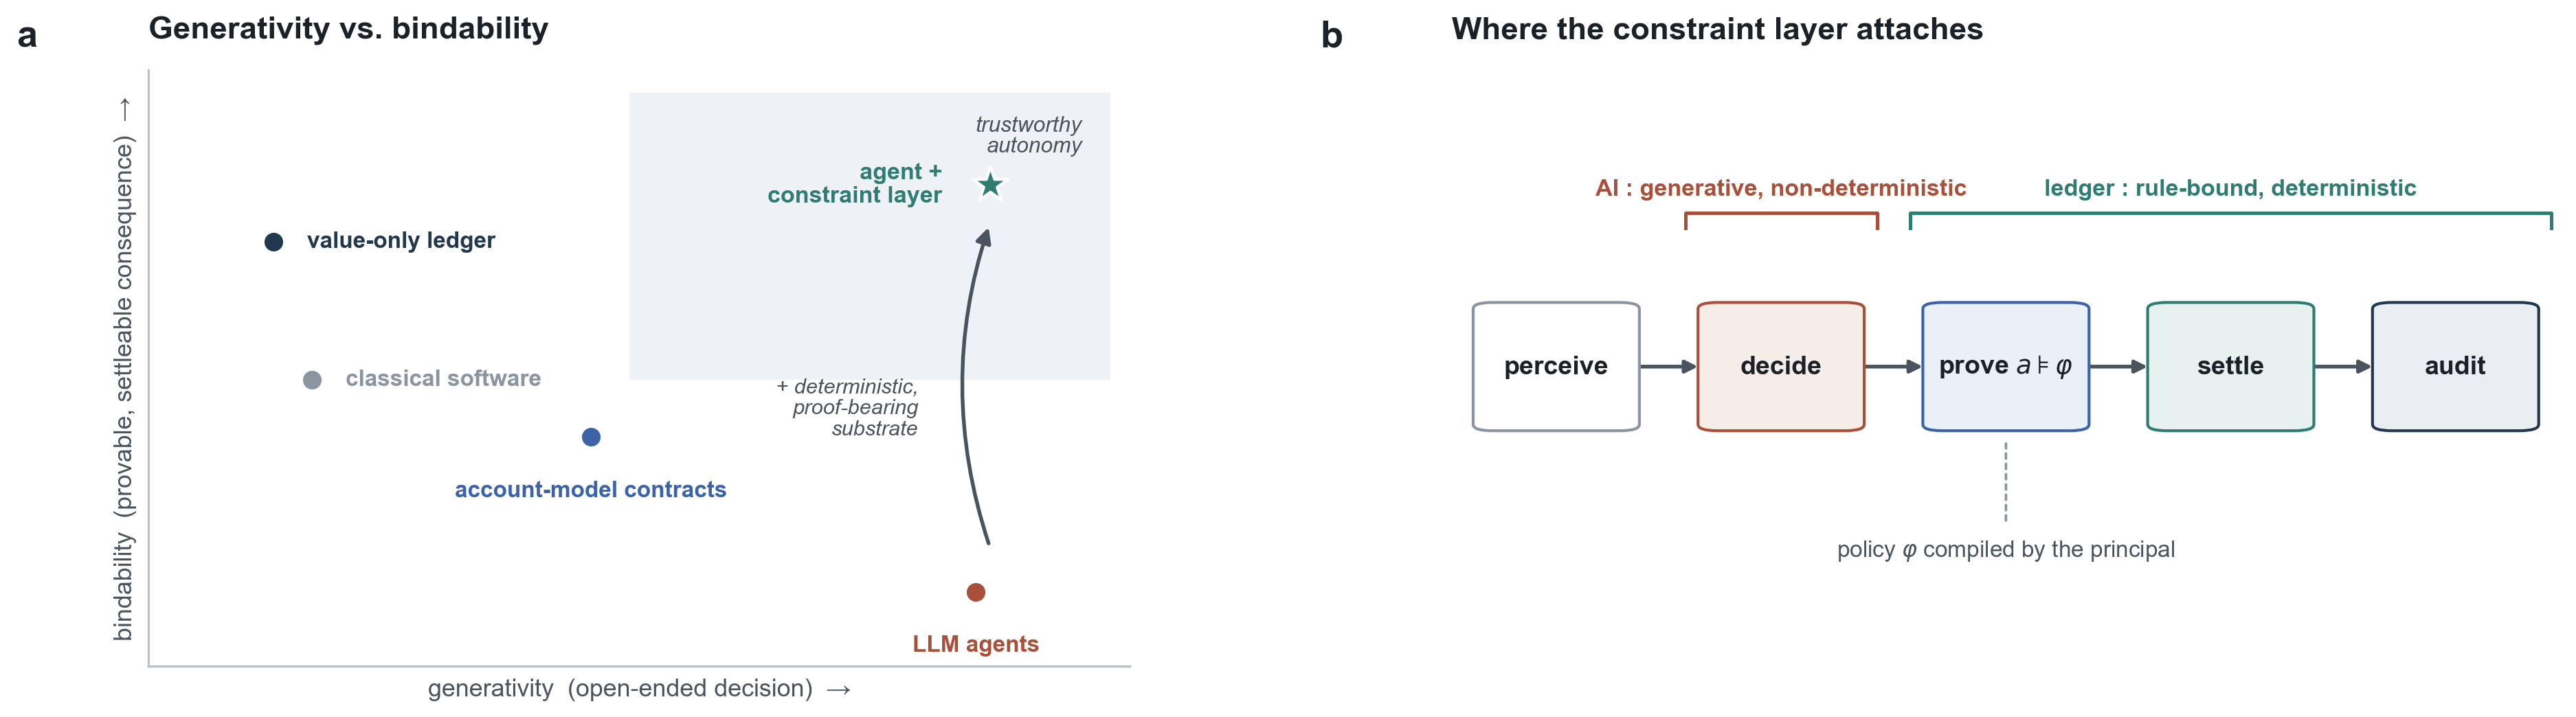
\includegraphics[width=\textwidth]{fig1_complementarity.png}
  \caption{互补性。\textbf{(a)}~按\emph{生成性}（开放式决策的能力）对\emph{可
    绑定性}（使决策可证、可清算、最终的能力）放置各系统。生成式智能体处于高
    生成性、近零可绑定性；仅记值账本与账户模型账本处于低生成性、部分可绑定
    性；目标——可信的自主性——只有将智能体与一个确定性的、自携证明的基底配
    对才能达到。\textbf{(b)}~智能体的动作生命周期。生成的、非确定的一步
    （\emph{决策}）属于模型；受规则约束的、确定的诸步（\emph{证明}、\emph{结
    算}、\emph{审计}）属于账本。约束层附着于二者边界，在此强制由委托人编译的
    策略谓词 $\varphi$。示意图。}
  \label{fig:complement}
\end{figure}

\begin{table}[t]
  \centering\small
  \caption{分工。智能体唯一的原生强项，正是账本唯一的原生弱项，反之亦然；承载
    后果的自主性需要两列同时具备。}
  \label{tab:division}
  \begin{tabular}{@{}lll@{}}
    \toprule
    能力 & 自主智能体 & 公共账本 \\
    \midrule
    开放式决策       & 原生         & 无 \\
    确定性 / 可重放   & 否           & 是 \\
    构造性规则绑定    & 仅建议       & 规则即代码 \\
    证明自身行为      & 只能断言     & 自携证明 \\
    不可逆结算        & 否           & 是 \\
    受界、可委托权限  & 无界         & 策略谓词 \\
    可问责身份        & 无抵押       & 密钥、公共记录 \\
    \bottomrule
  \end{tabular}
\end{table}

具体地读，基底执行智能体所不能的四项功能。\emph{它在事前约束。}一个动作可以被
做成携带一份证明，证明它满足委托人的策略——这笔转移在预算内、这个对手方被许
可、这次披露合法——由接收方在其生效前核查，沿袭「自携证明的代码」的谱系：生
产者把不受信的指令连同其安全性证明一并交付，消费者核查证明而非信任生产者
\citep{necula1997pcc}。智能体的权限于是成为陌生人可以验证的对象，而非委托人寄
望的某种秉性。\emph{它结算。}在确定性基底上，被核查的动作就是成为最终的动作，
中间没有可供修订的缝隙。\emph{它把合规变成谓词。}由于证明可以是零知识的，智能
体能证明自己满足某条规则而不暴露其背后的数据
\citep{goldwasser1989knowledge,bensasson2014zerocash}——越过辖区门槛、持有足
额抵押、已成年——于是结算携带对手方所需的证据、且仅此而已，验证不再是监控。
\emph{它原生地承载被委托的权限。}支撑这件事的机制正在被标准化：智能体支付协议
把一笔购买锚定到一串密码学签名的\emph{授权凭证（mandate）}——意图、购物车、支
付——使权限建立在「委托人批准了什么」的可验证、不可抵赖的证据之上，而非建立在
模型的概率性输出之上 \citep{ap2google2025}；一套 HTTP 原生方案让智能体在一次交
互中为资源付费并附上支付证明 \citep{x402coinbase2025}；带会话密钥的账户抽象则让
委托人铸造一份只限于某个对手方、某个金额、某段短有效期的凭证，边界在执行时被强
制而非被信任 \citep{erc4337}。智能合约在
多年前就供给了所缺的词汇——把合同条款表示为可执行对象
\citep{szabo1997formalizing}——而它所带来的验证成本下降，是这项技术的原始经济
性之一 \citep{catalini2020simple}。要点不在于其中任何一项孤立地说是新的；而在
于，组装起来，它恰恰是智能体所缺的那项后果的能力。

\section{账本要绑定一个智能体须成为什么}
\label{sec:requirements}

「一个账本」太过笼统。一个意在大规模绑定智能体的基底，必须同时满足五项要求；
缺其一，要么智能体逃出约束，要么一个可信第三方被悄悄重新引入到下一层——只是
排版更精美。诸要求从第一性原理陈述；\S\ref{sec:case} 以一个已部署系统对照之，
表~\ref{tab:requirements} 给出映射。

\paragraph{\R{1} —— 可证安全的共识。}
一个以「核查这个」取代「信我」为业的基底，不能把自身的安全性建立在「运营者看
起来诚实」之上。基础层的安全本身必须是一个可核查的主张，化归为既述假设与敌手
模型并加以证明——正如那些在显式同步与腐化假设下确立其保证的权益证明协议
\citep{kiayias2017ouroboros,david2018praos}。一个以声誉担保的后果层是种类上的
自相矛盾：它要求智能体的对手方去做这层本应替他们省去的那件事。

\paragraph{\R{2} —— 确定性结算：核查即清算。}
智能体证明有效的那个动作，必须就是被清算的那个动作。若一笔交易的效果取决于打
包时刻的全局状态——取决于同区块还落进了什么、以何种次序——那么本地核查的结
果与全局清算的结果就会分叉，而这道缝隙会被收割：抢跑、夹击、在决策与最终性之
间被抽取的价值 \citep{daian2020flashboys}。对人类交易者这是一笔成本；对以机器
速度交易的智能体则是致命的，因为它的合规证明是针对一个在结算时已不再成立的状
态算出的。本地验证必须等于全局状态转移（图~\ref{fig:delegation}b），否则约束
是针对一个不会到来的世界做出的核查。

\paragraph{\R{3} —— 富表达力、保护隐私的证明。}
基底必须能表达谓词，而不只是转移，并且必须允许它们在不披露的情况下被证明——
否则合规是以监控换来的，而一个为委托人行动的智能体会在每次动作中泄露委托人的
仓位、对手方与策略。它还必须可组合：证明之证明，使核查系统自身的历史不至于又
成为无界的工作量。私密智能合约的理论基础把这一点落到实处
\citep{kerber2021kachina}，而同构的链下执行让同样的规则在规模上运行、并如同在
基础层上算出那样返回 \citep{chakravarty2021hydra}。

\paragraph{\R{4} —— 无所有者的经济。}
排序、存储与可用性总要有人买单。若由一家公司买单，这家公司便能审查与两面陈
述，约束层于是沦为一个多了几道手续的私有数据库——可信第三方被重建。基底因此
需要一种内部资源，向一个无许可的群体购买安全与运营
\citep{nakamoto2008,brunjes2020rewards}；这——而非投机——才是原生资产承重的
角色。有所有者的验证者是公证人；有自筹资金公地的验证者才是基础设施。

\paragraph{\R{5} —— 能自我修订的规则。}
谓词、证明系统与参数都将改变；密码学会老化，政策有争议。不可修订的基底会僵
化；由基金会或公司修订的基底则有主（又是 \R{4}，上移一层）。剩下的选项是宪法
式的：通过留痕的、受规则约束的链上程序修订，且该程序自身的正当性也可被核查
\citep{cip1694}。这是任何地方都最未定的一项要求，诚实的立场是：它是一个开放的
制度问题，而非已解的工程问题。

\begin{table}[t]
  \centering\small
  \setlength{\tabcolsep}{5pt}
  \caption{代理级约束层的五项要求：每项为委托方保障了什么，以及一个已部署实例
    （\S\ref{sec:case}）所用的机制。文献为一手设计文献。}
  \label{tab:requirements}
  \begin{tabular}{@{}llll@{}}
    \toprule
    & 要求 & 为委托方保障什么 & 机制（个案） \\
    \midrule
    \R{1} & 可证共识 & 基础层本身无须被信任 &
      Ouroboros PoS \citep{kiayias2017ouroboros,david2018praos} \\
    \R{2} & 确定性结算 & 核查的动作即清算的动作 &
      扩展 UTXO \citep{chakravarty2020eutxo} \\
    \R{3} & 私密可组合证明 & 合规而不泄露仓位 &
      Hydra；Kachina/Midnight \citep{chakravarty2021hydra,kerber2021kachina} \\
    \R{4} & 无主经济 & 无任何一方能审查该智能体 &
      质押奖励 \citep{brunjes2020rewards} \\
    \R{5} & 自我修订规则 & 授权语言可演进 &
      链上宪法 \citep{cip1694} \\
    \bottomrule
  \end{tabular}
\end{table}

这五项要求把整个领域分了类。仅记值的账本满足 \R{1} 与一种强形式的 \R{4}，却
彻底不满足 \R{3}：它无法表达智能体授权所用的谓词。主流的账户模型链富于表达，
却交出了 \R{2}——其依赖次序的执行正是可抽取价值的原生栖息地
\citep{daian2020flashboys}——于是智能体核查过的动作不是清算的动作。许可链与联
盟链通过放弃 \R{4} 来重获确定性与表达力：它们的验证者是具名且经准入的，而这恰
恰是智能体的对手方必须信任的那个可信第三方。而多数设计对 \R{5} 保持沉默。这五
项两两满足容易，同时满足很难；正因如此，任何一个联合解的存在都值得审视，而非
被假定。

\section{一个已部署的架构}
\label{sec:case}

我们以一个系统对照 \R{1}--\R{5}：Cardano，选择它，是因为其文档化的设计决策
——其中数项长期被批评为过度工程——与这五项的对应完整度罕见。这里的主张是架
构对应，不是市场胜利；个案的价值在于，它把「这五项能否同时满足？」从一个愿望
变成一个存在性问题，且至少有一个肯定的实例。我们依次检读诸要求，然后坦陈个案
的负债。

\paragraph{\R{1}}
共识层是一族权益证明协议，其安全性在显式的敌手模型下得到证明——先是同步、继
而是带自适应腐化的半同步 \citep{kiayias2017ouroboros,david2018praos}。方法论
意义高于密码学意义：一个出售「核查、勿信」的层，已把自身的基础层安全做成可核
查的主张而非一句保证，而这正是其对手方在上一层所依赖的纪律。

\paragraph{\R{2}}
账本模型把比特币的未花费输出纪律延伸到完整合约，同时保住其决定性性质：一笔交
易的有效性、效果与费用，由它自身的输入在本地、在提交之前确定
\citep{chakravarty2020eutxo}。智能体证明的就是链上清算的。为富表达共享状态而
优化的账户型架构恰恰交出了这一点，而「核查」与「清算」之间的分叉正被工业化抽
取 \citep{daian2020flashboys}。在本论题之下，确定性不是一种性能口味；它使一个
智能体的动作成为关于其自身效果的可证主张，而非投进一场它看不见的拍卖的出价。

\paragraph{\R{3}}
表达力分层到达，且不向非用户征税。链上脚本承载公开谓词；状态通道把计算\emph{
同构地}抬到链下，在同一语义下运行同样的脚本，使返回的结果如同在基础层上算出
\citep{chakravarty2021hydra}；而一个以私密智能合约理论为根基的伙伴网络
\citep{kerber2021kachina} 运行的谓词，能在只披露谓词本身的前提下证明合规
\citep{midnight2024}。这正是智能体授权所需的选择性披露体制：证明规则，保留仓
位。

\paragraph{\R{4}}
区块生产向一个无许可的质押池群体购买，奖励方案经工程化设计使其在多个独立运营
者处达到均衡 \citep{brunjes2020rewards}，协议开发则由链上金库出资。基底以自己
的资源为自己的中立性付费——这就是开放公地与如今以「企业级区块链」出售的联盟
出函服务之间的类差：后者有所有者，因而重新引入了智能体对手方必须信任的那一
方。

\paragraph{\R{5}}
自 2023 年起，该系统在一部经批准的宪法之下运行由受托代表、质押池运营者与宪法
委员会组成的链上治理，每一项动议都在公共记录上 \citep{cip1694}。这套安排年
轻，第一批宪法危机也已到来；这并不构成否决，因为 \R{5} 在任何地方都未被解决，
而此处要紧的是：修订程序坐落于被验证的记录\emph{之内}，而非紧邻的董事会里。

诚实的检读须陈明负债。基础层吞吐量远低于中心化轨道；证明系统带来真实的证明与
验证开销；应用层生态有目共睹地挣扎，采用落后于架构数年；\R{5} 的治理尚不成熟
且有争议。这些都未被本论题掩盖，也都不是本论题的主题：个案立足于五项\emph{要
求}的联合满足，而 \S\ref{sec:open} 写明了何种证据将推翻这一检读。

\section{智能体商业的形态}
\label{sec:commerce}

这些部件组合成单一的模式（图~\ref{fig:delegation}a）。委托人不把密钥交给智能
体；它编译一份策略 $\varphi$——支出上限、对手方类别、升级条件——而智能体的权
限\emph{就是} $\varphi$。智能体的每一个动作都携带一份证明，证明该动作满足
$\varphi$；对手方在行动前核查该证明，于是边界由受其保护的一方强制执行，而非靠
委托人寄望。结算发生在确定性轨道上，于是被验证的动作就是被做成最终的动作
（\R{2}）；又因为每一步都对照公共账本留痕，审计便不是争议之后的取证重构，而是
对早已在册的证明的一次重放。权限在\emph{事前}受界；问责在\emph{事后}机械化。

\begin{figure}[t]
  \centering
  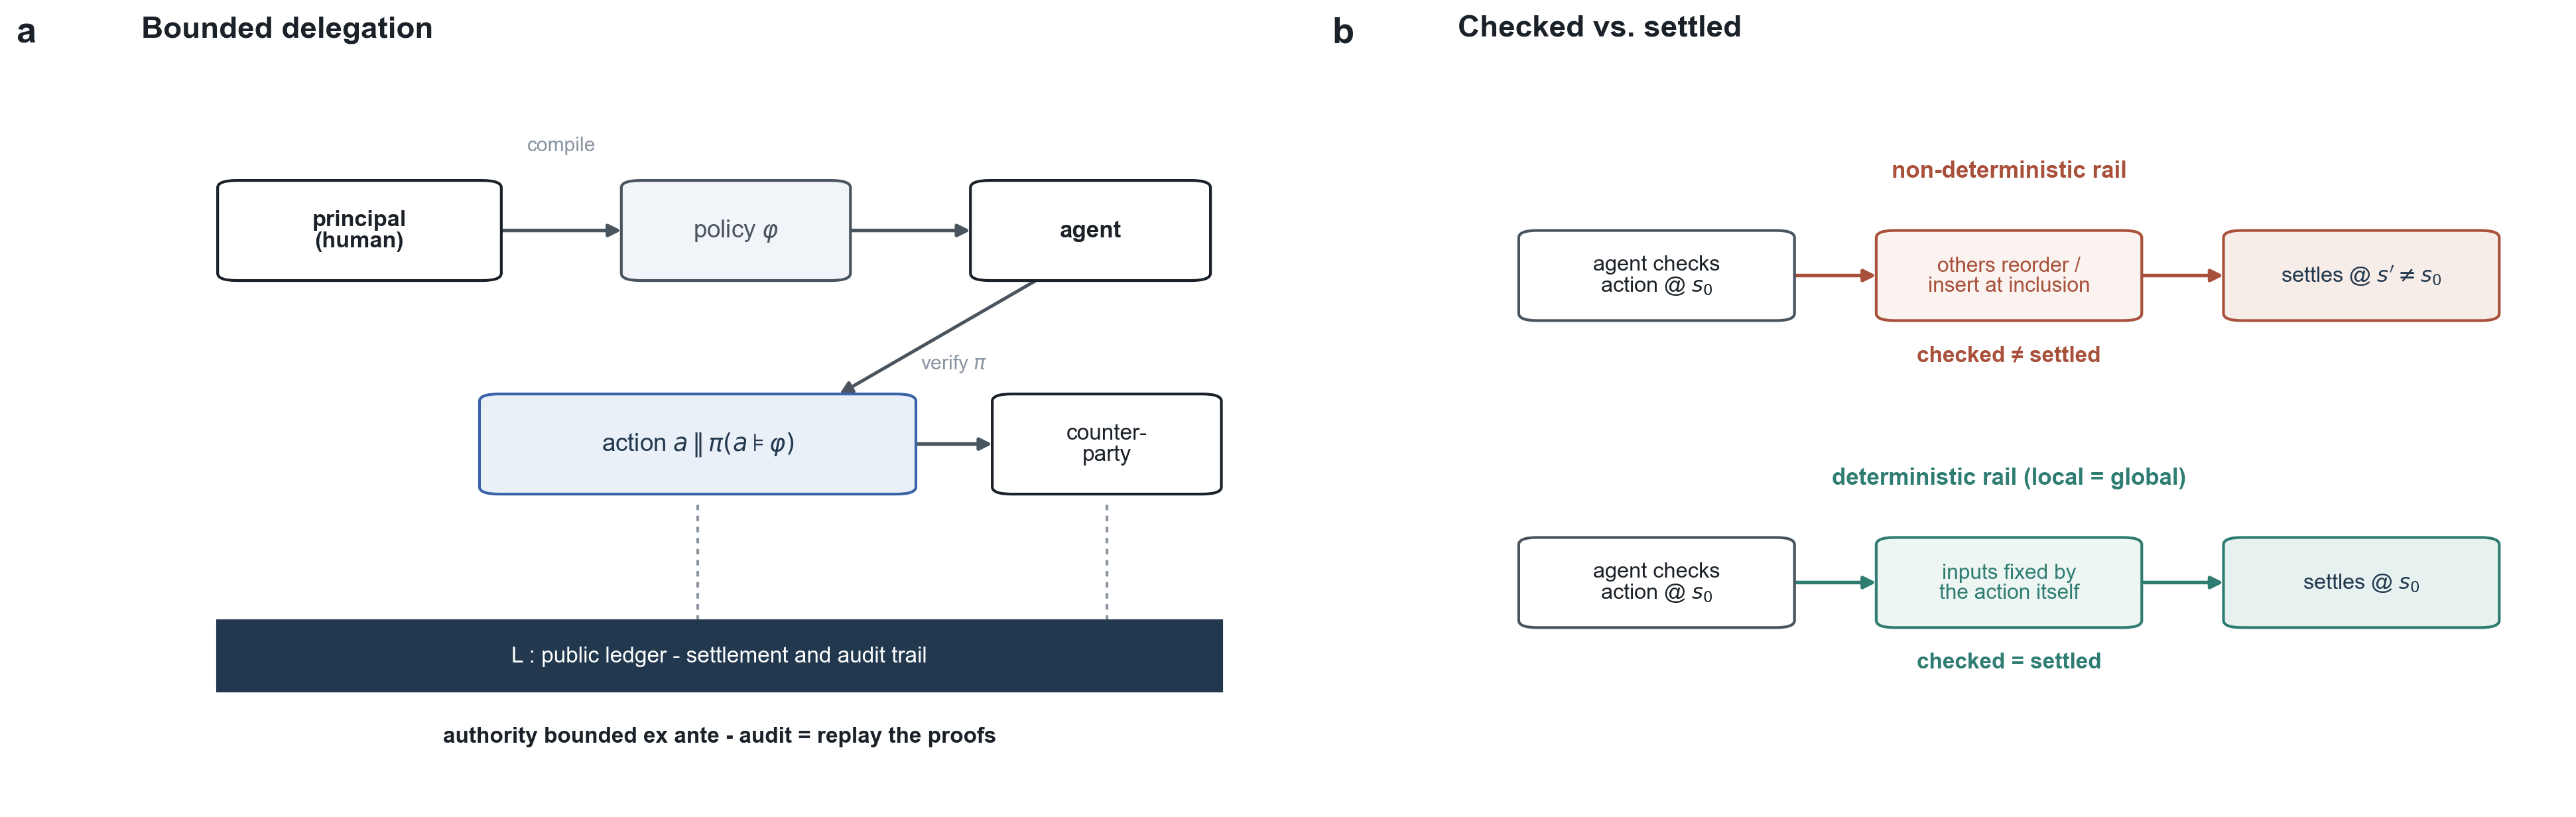
\includegraphics[width=\textwidth]{fig2_delegation.png}
  \caption{受界委托与确定性鸿沟。\textbf{(a)}~委托人编译策略 $\varphi$；智能体
    的动作 $a$ 携带证明 $\pi(a \models \varphi)$ 同行，由对手方核查；结算与审
    计化归为对照公共账本 $L$ 重放证明。权限在事前受界。\textbf{(b)}~为何确定性
    （\R{2}）承重：在非确定性轨道上，核查与打包之间的重排或插入会清算出一个状
    态 $s' \neq s_0$，于是智能体已验证的动作不是被清算的那个；在确定性轨道上，
    动作的输入固定其效果，核查即清算。示意图。}
  \label{fig:delegation}
\end{figure}

这不是关于智能体\emph{可能}如何交易的预测；它大致就是第一批标准已经声明的交易
方式。如今正在落地的智能体支付协议，把每一笔购买锚定到一串签名授权凭证，正是为
了让授权建立在可验证的意图、而非模型的一面之词之上
\citep{ap2google2025,x402coinbase2025}，而账户抽象提供了授权凭证所针对的那份受
界、可撤销的凭证 \citep{erc4337}。它们尚未提供的，是 \R{2} 的基底保证：它们多数
结算在账户模型轨道上，核查的动作与清算的动作仍可能分叉
\citep{daian2020flashboys}。互补关系的需求侧正在公开地被建造；能让它在机器速度下
安全的那份确定性，才是仍然缺失的一半，\S\ref{sec:open} 把它当作真正的检验来
对待。

身份沿同一条线分解。对手方必须回答的问题——\emph{这是什么，谁在背后？}——分
解为可核查的谓词。在需要之处，人格成为行为者可以证明而非断言之物
\citep{borge2017personhood}；智能体凭证通过来源本身可核查的签名回链至一个可问
责的委托人 \citep{diffie1976new}；而智能体所产之物的出处，可以作为一份签名的
主张随之同行，而不是留给某个检测器去事后猜疑 \citep{c2pa2024}。每一处，动作都
与定义整个架构的那个动作相同：以事前附着的证明，取代对一件流利人造物的事后判
断。

由此有两点观察。其一关乎成本。人类把这套机制体验为摩擦——密钥、钱包、出函，
一种比径直被信任更差的体验——这正是面向人类的加密始终难以要紧的原因。智能体
体验到的恰好相反：声誉是它们天生持有不了的东西，而生成与核查证明正是它们以原
生速度所做之事；它们不疲倦、不会看错地址，也无法通过一个只接纳有效动作的基底
被社会工程。那种把人类用户推开的摩擦，对正在到来的群体而言是无重量的。其二关
乎契合的方向。生成式 AI 是需求：它产出决策的速度，快过任何可信的人类机构所能
审核。可验证的、确定性的结算，是唯一一种吞吐量随算力而非随注意力扩展的供给回
应。二者不是争夺同一叙事位置的对手；一个使决策充裕，另一个使决策绑定——而一
个无法绑定的决策，在经济意义上，不过是空话。

\section{开放问题与可证伪}
\label{sec:open}

本论题是一个技术上的赌注，而一个诚实的赌注要同时写明它未解的部分，以及何种证
据将把它判输。

四个问题是开放的。\emph{成本与延迟}：为每一个动作出证并不免费，一个持续交易的
智能体可能产生证明的速度，快过它们能被廉价地生成或验证的速度；自携证明的结算
能否以可接受的成本满足机器速度的商业，尚无定论，而递归组合（\R{3}）是部分答
案，不是完成的答案。\emph{治理}（\R{5}）：在被验证的记录之内自我修订，尚且年
轻、参与稀薄、且已承压；没有任何系统证明过一部宪法能在既不被俘获也不陷入瘫痪
的情况下演进一套证明语言与一套费用政策。\emph{谓词问题}：一份授权的好坏，取决
于委托人实际能表达的策略 $\varphi$，而为开放式行为书写 $\varphi$——预先设想一
个智能体绝不可做之事——其难度可能不亚于它所类比的对齐问题；基底强制执行
$\varphi$，却不撰写它。\emph{自举}：约束层在智能体与对手方都已使用它时最有用，
这是经典的采用陷阱，架构上的适配并不能化解它。

四项观察将证伪这一论述。最早的智能体支付标准如今恰恰结算在非确定性轨道上
\citep{x402coinbase2025}；若智能体商业随规模增长仍滞留于此、不为可抽取价值之税
\citep{daian2020flashboys} 所动，那么 \R{2} 关于「智能体愿意付费去避免什么」的
判断就是错的，确定性并不承重。若出处与智能体身份聚拢为少数
平台出函服务——设备厂商、应用商店、模型供应商——那么无主基底（\R{4}）便输给
了一个重新中心化的方案，证词体制只是以更高的集中度、配上根密钥被重建；在我们
看来，这是本论题失败的最可能方式，而它是市场结构问题，不是可行性问题。若技术
进展使智能体在\emph{内部}变得可绑定——在模型栈自身之内承载硬件背书的、可验证
的执行——那么外部基底便是多余的，互补关系随之消解。又若在开放基底之间，为结
算、出证与出函所付费用的份额，始终未能超过为投机换手所付的份额，那么这些系统
就是赌场而非基础设施，无论其设计如何——\S\ref{sec:case} 的个案对这项检验，刻
意不予豁免。

\section{结语：谁来书写规则}
\label{sec:coda}

分工就是全部论证。一个生成式模型供给决策；一个确定性的、自携证明的、无主的基
底供给后果；二者合起来，造出一个可被委托、可受界、可问责的自主行为者——而任
一半单独都做不到。这不是一个机器取代制度的故事。这是一个为非人类行为者重建那
件制度曾为人类所做之事的故事：把一个决策转化为一个绑定的承诺。

有一种能力，在这道分工的两侧都不出现。基底强制执行策略 $\varphi$；智能体在其
内行动；但 $\varphi$ 的抉择——一个智能体绝不可做什么、什么算作合规、哪些结果
值得被做成不可逆——由两者皆非。书写规则不是一项可委托给智能体的任务，因为它
正是界定其下每一次委托之边界的那个动作；它也不是基底执行的一项计算，因为基底
只核查。它是约束的撰写，并停留在那个承担「写错了的后果」的人身上。当决策变得
充裕、其结算变得自动，稀缺而承载后果的动作便不再是决策，也不再是执行。它是：
预先地、并留诸记录地，言明什么应当、什么不应当被允许绑定。

\paragraph*{数据可得性}
本文为理论贡献；不报告任何实验、任何实证数据集。所有主张均依托于所引文献；复现插图所需的脚本与材料随代码一并发布。

\paragraph*{代码可得性}
两幅插图均为示意图，由公开发布于 \url{https://github.com/xinhao-zheng/constraint-layer}
的脚本生成；未绘制任何经验序列。

\paragraph*{作者贡献}
X.Z. 构思论证、设计插图并撰写全文。

\paragraph*{利益冲突}
作者不持有文中讨论的任何资产头寸，亦未接受任何被提及实体的资助。

\paragraph*{伦理说明}
不涉及人类受试者。系统与产品名称仅作描述性使用；个案分析是架构性的，不构成投
资建议。
\begin{thebibliography}{27}
\small\setlength{\itemsep}{2pt}
% 条目按正文首次引用顺序排列。

\bibitem[North(1990)]{north1990institutions}
North, D.~C. (1990). \emph{Institutions, Institutional Change and
Economic Performance}. Cambridge University Press.

\bibitem[Arrow(1974)]{arrow1974limits}
Arrow, K.~J. (1974). \emph{The Limits of Organization}. Norton, New York.

\bibitem[Park et~al.(2023)]{park2023generative}
Park, J.~S., O'Brien, J.~C., Cai, C.~J., Morris, M.~R., Liang, P., and
Bernstein, M.~S. (2023). Generative agents: Interactive simulacra of
human behavior. In \emph{UIST 2023}. ACM.

\bibitem[Chan et~al.(2023)]{chan2023harms}
Chan, A., Salganik, R., Markelius, A., et~al. (2023). Harms from
increasingly agentic algorithmic systems. In \emph{ACM FAccT 2023},
pages 651--666.

\bibitem[Sadasivan et~al.(2023)]{sadasivan2023detection}
Sadasivan, V.~S., Kumar, A., Balasubramanian, S., Wang, W., and Feizi, S.
(2023). Can {AI}-generated text be reliably detected? arXiv:2303.11156.

\bibitem[Zhang et~al.(2023)]{zhang2023watermarks}
Zhang, H., Edelman, B.~L., Francati, D., Venturi, D., Ateniese, G., and
Barak, B. (2023). Watermarks in the sand: Impossibility of strong
watermarking for generative models. arXiv:2311.04378.

\bibitem[Necula(1997)]{necula1997pcc}
Necula, G.~C. (1997). Proof-carrying code. In \emph{POPL~'97}, pages
106--119. ACM.

\bibitem[Goldwasser et~al.(1989)]{goldwasser1989knowledge}
Goldwasser, S., Micali, S., and Rackoff, C. (1989). The knowledge
complexity of interactive proof systems. \emph{SIAM Journal on
Computing}, 18(1):186--208.

\bibitem[Ben-Sasson et~al.(2014)]{bensasson2014zerocash}
Ben-Sasson, E., Chiesa, A., Garman, C., Green, M., Miers, I., Tromer, E.,
and Virza, M. (2014). Zerocash: Decentralized anonymous payments from
{Bitcoin}. In \emph{IEEE Symposium on Security and Privacy}, pages
459--474.

\bibitem[Google et~al.(2025)]{ap2google2025}
Google and partners (2025). \emph{Agent Payments Protocol (AP2): An Open
Protocol for Agent-Led Payments}. Technical specification, September 2025.

\bibitem[Coinbase and Cloudflare(2025)]{x402coinbase2025}
Coinbase and Cloudflare (2025). \emph{x402: An Open Standard for
Internet-Native Payments over {HTTP} 402}. x402 Foundation.

\bibitem[Buterin et~al.(2021)]{erc4337}
Buterin, V., Weiss, Y., Tirosh, D., Nacson, S., and Forshtat, A. (2021).
{ERC-4337}: Account abstraction using an alt mempool. Ethereum
Improvement Proposals.

\bibitem[Szabo(1997)]{szabo1997formalizing}
Szabo, N. (1997). Formalizing and securing relationships on public
networks. \emph{First Monday}, 2(9).

\bibitem[Catalini and Gans(2020)]{catalini2020simple}
Catalini, C. and Gans, J.~S. (2020). Some simple economics of the
blockchain. \emph{Communications of the ACM}, 63(7):80--90.

\bibitem[Kiayias et~al.(2017)]{kiayias2017ouroboros}
Kiayias, A., Russell, A., David, B., and Oliynykov, R. (2017). Ouroboros:
A provably secure proof-of-stake blockchain protocol. In \emph{CRYPTO
2017}, LNCS 10401, pages 357--388. Springer.

\bibitem[David et~al.(2018)]{david2018praos}
David, B., Ga\v{z}i, P., Kiayias, A., and Russell, A. (2018). Ouroboros
Praos: An adaptively-secure, semi-synchronous proof-of-stake blockchain.
In \emph{EUROCRYPT 2018}, LNCS 10821, pages 66--98. Springer.

\bibitem[Daian et~al.(2020)]{daian2020flashboys}
Daian, P., Goldfeder, S., Kell, T., Li, Y., Zhao, X., Bentov, I.,
Breidenbach, L., and Juels, A. (2020). Flash boys 2.0: Frontrunning in
decentralized exchanges, miner extractable value, and consensus
instability. In \emph{IEEE Symposium on Security and Privacy}, pages
910--927.

\bibitem[Chakravarty et~al.(2020)]{chakravarty2020eutxo}
Chakravarty, M. M.~T., Chapman, J., MacKenzie, K., Melkonian, O.,
Peyton~Jones, M., and Wadler, P. (2020). The extended {UTXO} model. In
\emph{Financial Cryptography Workshops (WTSC)}, LNCS 12063, pages
525--539. Springer.

\bibitem[Chakravarty et~al.(2021)]{chakravarty2021hydra}
Chakravarty, M. M.~T., Coretti, S., Fitzi, M., Ga\v{z}i, P., Kant, P.,
Kiayias, A., and Russell, A. (2021). Hydra: Fast isomorphic state
channels. Cryptology ePrint Archive, Report 2020/299.

\bibitem[Kerber et~al.(2021)]{kerber2021kachina}
Kerber, T., Kiayias, A., and Kohlweiss, M. (2021). Kachina: Foundations
of private smart contracts. In \emph{IEEE Computer Security Foundations
Symposium}, pages 47--62.

\bibitem[Midnight(2024)]{midnight2024}
Midnight Foundation (2024). \emph{Midnight: A Data-Protection
Blockchain---Technical Overview}. Project documentation.

\bibitem[Nakamoto(2008)]{nakamoto2008}
Nakamoto, S. (2008). Bitcoin: A peer-to-peer electronic cash system.
White paper.

\bibitem[Br\"unjes et~al.(2020)]{brunjes2020rewards}
Br\"unjes, L., Kiayias, A., Koutsoupias, E., and Stouka, A.-P. (2020).
Reward sharing schemes for stake pools. In \emph{IEEE European Symposium
on Security and Privacy}, pages 256--275.

\bibitem[CIP-1694(2023)]{cip1694}
Cardano community (2023). \emph{CIP-1694: An On-Chain Decentralized
Governance Mechanism for Voltaire}. Cardano Improvement Proposals.

\bibitem[Borge et~al.(2017)]{borge2017personhood}
Borge, M., Kokoris-Kogias, E., Jovanovic, P., Gasser, L., Gailly, N., and
Ford, B. (2017). Proof-of-personhood: Redemocratizing permissionless
cryptocurrencies. In \emph{IEEE EuroS\&P Workshops}, pages 23--26.

\bibitem[Diffie and Hellman(1976)]{diffie1976new}
Diffie, W. and Hellman, M.~E. (1976). New directions in cryptography.
\emph{IEEE Transactions on Information Theory}, 22(6):644--654.

\bibitem[C2PA(2024)]{c2pa2024}
Coalition for Content Provenance and Authenticity (2024). \emph{C2PA
Technical Specification, v2.0}. Standard.

\end{thebibliography}

\end{document}
